%% ----------------------------------------------------------------
%% main.tex -- Proyecto Final Tecnólogo en Mecatrónica (UTEC Uruguay)
%% Adaptado al template oficial UTEC ITR Suroeste, Fray Bentos
%% ----------------------------------------------------------------

\documentclass[a4paper, 12pt, oneside]{tesisutec}

\graphicspath{{images/}}
\usepackage{grffile}

\usepackage[square, numbers, comma, sort&compress]{natbib}
\usepackage{verbatim}
\hypersetup{urlcolor=blue, colorlinks=true}

\usepackage[utf8]{inputenc}

%% ============================================================================
%% METADATOS - Datos extraídos del documento version_previa
%% ============================================================================
\title{DISEÑO Y CONSTRUCCIÓN DE UN ROBOT DE TIPO COLABORATIVO (COBOT) CON CAPACIDAD DE AGARRE CON VENTOSA}
\author{Raul Benelli}
\authorii{Valentin Morales}
\authorci{3.865.265-9}
\authorciii{4.949.690-3}
\email{correo@ejemplo.com}
\codigoproyecto{PTM24008}
\supervisor{Diego Quiroga}
\cotutor{Ivan Elgue}
\date{Noviembre 2024}

%% ============================================================================
\begin{document}

\frontmatter
\maketitle
\setstretch{1.5}

% Declaración de autoría (obligatoria)
%% ============================================================================
%% Declaración de autoría (según template oficial UTEC)
%% Para un autor: defina solo \author y \authorci
%% Para dos autores: defina también \authorii y \authorciii
%% ============================================================================

\makeatletter
\ifx\authornameii\@empty
  \declaracionautoria{%
  Yo, \authornames, con documento de identidad \authorcino, estudiante del Tecnólogo en Mecatrónica de UTEC \itrname\ \sedename, en relación al Proyecto Final titulado ``\@title'', código \codigoproy, para su defensa y evaluación, declaro la autoría y originalidad del mismo, así mismo, que todas las fuentes de información que han sido citadas o utilizadas como argumento de este trabajo están referenciadas en él y fueron incluidas en las Referencias Bibliográficas.
  }
\else
  \declaracionautoria{%
  \authornames\ e \authornameii, con documento de identidad \authorcino\ y \authorcinoii, respectivamente, estudiantes del Tecnólogo en Mecatrónica de UTEC \itrname\ \sedename, en relación al Proyecto Final titulado ``\@title'', código \codigoproy, para su defensa y evaluación, declaramos la autoría y originalidad del mismo, así mismo, que todas las fuentes de información que han sido citadas o utilizadas como argumento de este trabajo están referenciadas en él y fueron incluidas en las Referencias Bibliográficas.
  }
\fi
\makeatother


% Agradecimientos
%% ============================================================================
%% Agradecimientos
%% ============================================================================

\acknowledgements{%
Se deben redactar de manera formal, mencionando a las instituciones o personas que contribuyeron y apoyaron la realización de la investigación.

% Agradecer a los tutores Diego Quiroga e Ivan Elgue, a UTEC, a los compañeros, etc.
}


% Resumen y Abstract
%% ============================================================================
%% Resumen (máx. 250 palabras según template oficial)
%% ============================================================================

\resumen{%
Este trabajo presenta el diseño y construcción de un robot colaborativo (cobot) con capacidad de agarre mediante ventosa, utilizando servomotores Herkulex DRS-0602 y el gripper piCOBOT. El proyecto se desarrolló en el marco del Tecnólogo en Mecatrónica de UTEC ITR Suroeste, con el objetivo de impulsar la adopción de robótica colaborativa y fortalecer el aprendizaje práctico. Se analizaron los aspectos mecánicos, eléctricos y electrónicos necesarios para el diseño; se desarrolló una librería propia para el control de los motores DRS-0602 ante la ausencia de soporte adecuado; y se construyó un prototipo de 4 grados de libertad mediante impresión 3D en PLA. La estructura modular, el sistema de comunicación UART y el diseño colaborativo (bordes redondeados, limitación de velocidades) permitieron validar el funcionamiento del cobot como plataforma demostrativa. Los resultados confirman la viabilidad de integrar componentes comerciales accesibles en un brazo robótico colaborativo de escritorio, con potencial para futuras mejoras en materiales, control embebido e interfaz de usuario.

\textbf{Palabras clave:} cobot; robótica colaborativa; Herkulex DRS-0602; piCOBOT; impresión 3D; industria 4.0.
}

%% ============================================================================
%% Abstract (versión en inglés del resumen)
%% ============================================================================

\abstract{%
This work presents the design and construction of a collaborative robot (cobot) with vacuum gripping capability, using Herkulex DRS-0602 servomotors and the piCOBOT gripper. The project was developed within the Mechatronics Technologist program at UTEC ITR Suroeste, with the aim of promoting the adoption of collaborative robotics and strengthening hands-on learning. Mechanical, electrical and electronic aspects required for the design were analyzed; a custom library was developed for DRS-0602 motor control due to lack of adequate support; and a 4-degree-of-freedom prototype was built using 3D printing in PLA. The modular structure, UART communication system and collaborative design (rounded edges, speed limits) allowed validation of the cobot as a demonstrative platform. The results confirm the feasibility of integrating accessible commercial components into a desktop collaborative robotic arm, with potential for future improvements in materials, embedded control and user interface.

\textbf{Key words:} cobot; collaborative robotics; Herkulex DRS-0602; piCOBOT; 3D printing; Industry 4.0.
}


% Índice
\tableofcontents
\addtocontents{toc}{\vspace{1.5em}}

%% ============================================================================
\mainmatter
\pagestyle{fancy}

% Capítulos
%% ============================================================================
%% CAPÍTULO 1 - EL PROBLEMA
%% ============================================================================

\chapter{EL PROBLEMA}

\section{Planteamiento del problema}

Los robots colaborativos (cobots) son una tecnología emergente que está revolucionando la industria 4.0, gracias a su capacidad de operar de manera segura y eficiente junto a los seres humanos. Esta característica clave ha permitido no solo avanzar hacia la automatización de procesos, sino también consolidar el concepto de la industria 5.0, donde la colaboración humano-máquina es más estrecha y fluida.

En este contexto, el diseño y desarrollo de un cobot dentro de la Universidad Tecnológica del Uruguay (UTEC) no solo impulsará la adopción de esta tecnología, sino que también generará beneficios significativos. Entre estos se incluyen la creación de nuevos proyectos de investigación en robótica colaborativa y el fortalecimiento del aprendizaje práctico de los estudiantes de ingeniería en mecatrónica.

Los cobots se destacan por su flexibilidad, tamaño reducido y fácil integración en diversos entornos laborales. Sin embargo, diseñar y construir un cobot presenta varios desafíos técnicos. Estos incluyen la selección adecuada de componentes mecánicos, eléctricos y electrónicos, así como la integración efectiva de sistemas de control. En este proyecto se plantea el uso del motor DRS 0602, conocido por su precisión y rápida capacidad de respuesta, como solución para la propulsión del cobot. Además, se utilizará el gripper piCOBOT, que está diseñado específicamente para aplicaciones colaborativas y ofrece una solución eficaz para la manipulación de objetos. La integración de estos componentes requiere un análisis en profundidad de todos los aspectos mecánicos y electrónicos, y un diseño cuidadoso de la estructura y el sistema de control del cobot.

Además de ser una justificación técnica y académica, este proyecto representa una valiosa oportunidad para nosotros como estudiantes de ingeniería en mecatrónica. Nos permite aplicar y desarrollar los conocimientos adquiridos a lo largo de nuestra formación académica en un entorno práctico. Al enfrentar estos retos, podremos adquirir competencias clave en robótica colaborativa y tecnologías emergentes, contribuyendo así al progreso del sector y a la transición de sistemas de producción actuales hacia la industria 4.0.

\section{Objetivos}

\subsection{Objetivo General}

Diseñar y construir un cobot (robot colaborativo) utilizando el motor DRS 0602 y el gripper piCOBOT.

\subsection{Objetivos Específicos}

\begin{enumerate}
  \item Analizar los aspectos mecánicos, eléctricos y electrónicos relevantes para el diseño y funcionamiento del robot.
  \item Diseñar la estructura del robot y un sistema básico de control integrando un sistema embebido, considerando aspectos de robótica colaborativa.
  \item Construir la estructura y la electrónica, integrando todos los componentes necesarios para el funcionamiento del robot colaborativo.
  \item Verificar el funcionamiento de la estructura y el sistema de control para el robot colaborativo con los motores DRS 0602 y el gripper piCOBOT.
\end{enumerate}

\section{Alcance, limitaciones y beneficiarios}

\subsection{Alcance}

% Completar según el documento original.
Describa aquí el alcance del proyecto.

\subsection{Limitaciones}

% Completar según el documento original.
Describa aquí las limitaciones encontradas.

%% ============================================================================
%% CAPÍTULO 2 - MARCO TEÓRICO
%% ============================================================================

\chapter{MARCO TEÓRICO}

\section{Antecedentes de la investigación}

\cite{delacruz2022} presentó su proyecto titulado ``Diseño mecánico de un robot colaborativo móvil usando un sistema de engranajes planetarios''. Este trabajo se centró en el diseño mecánico de un robot colaborativo móvil, sin implementación de prototipo físico, utilizando engranajes planetarios que permiten una transmisión eficiente de par y velocidad en el brazo robótico. Este diseño no solo considera la geometría de los engranajes, sino también los ejes que los soportan, optimizando así su estabilidad y durabilidad. Dado su potencial para implementación y fabricación, el proyecto se planteó como una de las etapas iniciales de un sistema colaborativo móvil, proponiéndose en futuros trabajos el desarrollo físico y prototipo real del diseño. Este sistema planetario destaca por su diseño compacto, que distribuye el par en múltiples puntos a través de satélites, logrando una mayor transmisión de par sin pérdida significativa de velocidad.

\section{Cobot (Robot Colaborativo)}

Un robot colaborativo es un robot que se puede utilizar en una operación colaborativa, en la que un sistema robótico diseñado específicamente y un operador humano trabajan en cooperación directa dentro de un espacio de trabajo definido. El término robot define el brazo robótico y el control del robot y no incluye el efector final o la pieza del robot. Con el término sistema robótico describimos robot, efector final y pieza de trabajo \cite{lenarcic2012}.

Las características operativas de los sistemas de robots colaborativos son significativamente diferentes de las de los sistemas de robots industriales tradicionales presentados en las normas ISO 10218-1:2011 e ISO 10218-2:2011. En las operaciones de robots colaborativos, los operadores pueden trabajar en proximidad directa al sistema de robot mientras el sistema está activo, y el contacto físico entre un operador y el sistema de robot puede ocurrir dentro del espacio de trabajo colaborativo. Como tal, se deben introducir medidas de protección adecuadas para los sistemas de robots colaborativos \cite{lenarcic2012}.

\begin{figure}[htbp]
  \centering
  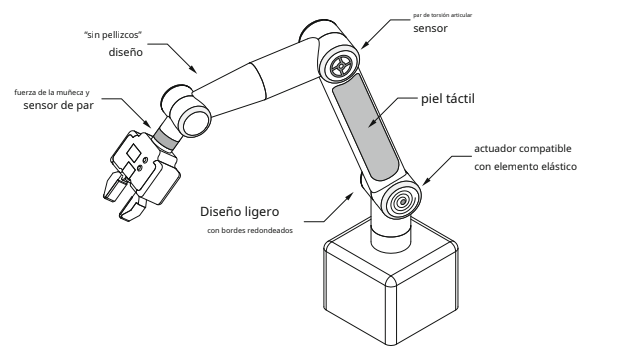
\includegraphics[width=0.6\textwidth]{Esquema del robot paralelo de 6 grados de libertad..png}
  \caption{Esquema del robot paralelo de 6 grados de libertad. Extraído de \cite{lenarcic2012}.}
  \label{fig:robot-paralelo}
\end{figure}

\section{Evolución de la robótica colaborativa}

El desarrollo de robots colaborativos (cobots) ha experimentado una importante evolución desde su surgimiento hasta convertirse en una de las tecnologías clave dentro de la Industria 4.0 y la emergente Industria 5.0. La historia de los cobots comienza en los años 90, cuando el concepto de robots que pudieran interactuar de manera segura y directa con los humanos comenzó a desarrollarse como una solución a las limitaciones de los robots industriales tradicionales.

Los robots industriales convencionales, introducidos por primera vez en la década de 1960, fueron diseñados principalmente para realizar tareas repetitivas y peligrosas en entornos de manufactura pesada. Estos robots, como los brazos robóticos utilizados en líneas de montaje automotriz, estaban confinados a áreas aisladas para evitar cualquier interacción peligrosa con los trabajadores humanos. Si bien estos robots lograron aumentar la eficiencia en la producción, su incapacidad para colaborar directamente con los humanos limitaba su flexibilidad en entornos cambiantes o donde se requería la intervención humana.

En 1996, el primer ``cobot'' fue desarrollado por J. Edward Colgate y Michael Peshkin en la Northwestern University. A diferencia de los robots industriales tradicionales, los cobots están diseñados para compartir espacios de trabajo con humanos de manera segura, aprovechando su capacidad para interactuar físicamente con las personas en tareas colaborativas. Estos primeros cobots no funcionan de manera autónoma; en cambio, asistían a los operadores humanos con tareas como guiar herramientas pesadas o manipular piezas de gran tamaño, permitiendo a los trabajadores realizar sus labores con mayor precisión y menor esfuerzo físico.

Con el avance de la tecnología y la llegada de la Industria 4.0, caracterizada por la automatización avanzada, la interconectividad y el uso de datos en tiempo real, los cobots encontraron un entorno ideal para su adopción masiva. La Industria 4.0 impulsó la integración de sistemas ciberfísicos, el Internet de las Cosas (IoT) y el análisis de datos en procesos de producción, lo que permitió a los cobots operar de manera más inteligente, flexible y eficiente. A diferencia de los robots tradicionales, que requerían programación especializada y compleja, los cobots modernos se caracterizan por su facilidad de programación y su capacidad para aprender nuevas tareas mediante interfaces intuitivas.

Más recientemente, la evolución de los cobots ha tomado un giro hacia la Industria 5.0, un concepto emergente que se centra en la personalización masiva y la interacción más cercana entre humanos y máquinas. A diferencia de la Industria 4.0, que enfatiza la automatización completa, la Industria 5.0 busca una colaboración más profunda entre humanos y robots, donde las habilidades humanas, como la creatividad y la toma de decisiones, se combinan con la precisión y eficiencia de los cobots.

\section{Operación colaborativa}

La operación colaborativa no se define únicamente con el uso del robot, sino que está condicionada por la tarea, lo que está haciendo el sistema robótico y el espacio en el que se realiza la tarea. Se pueden incluir cuatro técnicas principales (una o una combinación de más) en la operación colaborativa:
\begin{itemize}
  \item Parada monitoreada con clasificación de seguridad;
  \item Guía manual;
  \item Monitoreo de velocidad y separación;
  \item Limitación de potencia y fuerza.
\end{itemize}

Con las cuatro técnicas, el robot trabaja en modo automático. Los detalles principales de los cuatro métodos se presentan en la Tabla~\ref{tab:operaciones-colab} \cite{lenarcic2012}.

\begin{table}[htbp]
  \centering
  \caption{Tabla de tipos de operaciones colaborativas. Información adaptada de \cite{lenarcic2012}.}
  \label{tab:operaciones-colab}
  \begin{tabular}{ll}
    \toprule
    Técnica & Descripción \\
    \midrule
    Parada monitoreada & Ningún movimiento en presencia del operador \\
    Guía manual & Movimiento únicamente por operador directo \\
    Velocidad y separación & Contacto impedido entre robot y operador \\
    Limitación de potencia & El robot no puede impartir fuerza excesiva \\
    \bottomrule
  \end{tabular}
\end{table}

\subsection{Guía manual}

Para guiarlo manualmente, el robot debe estar equipado con un dispositivo de guía especial ubicado en el efector final del robot o cerca de él, que sirve para transmitir comandos de movimiento al sistema del robot. El dispositivo debe incorporar una parada de emergencia y un dispositivo de habilitación, a menos que el sistema del robot cumpla con medidas de diseño inherentemente seguras o funciones de limitación de seguridad \cite{lenarcic2012}.

\begin{figure}[htbp]
  \centering
  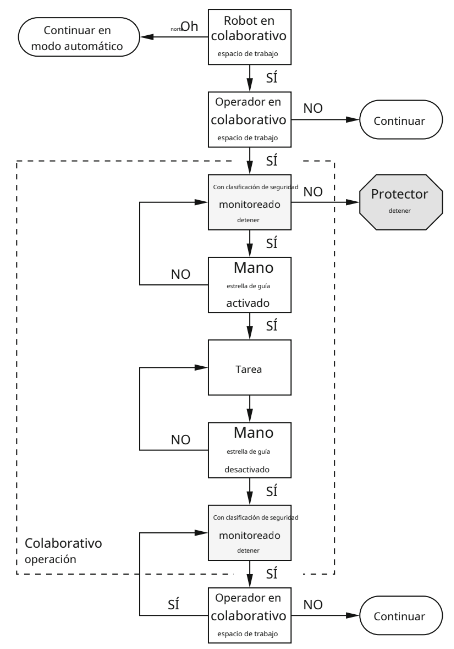
\includegraphics[width=0.6\textwidth]{diag_secuencia operativa.png}
  \caption{Secuencia operativa para el guiado manual. Información adaptada de \cite{lenarcic2012}.}
  \label{fig:guia-manual}
\end{figure}

\subsection{Monitoreo de velocidad y separación}

En este método, el operador y el sistema robótico pueden moverse simultáneamente en el espacio de trabajo colaborativo. Durante las operaciones conjuntas, se mantiene en todo momento la distancia mínima de separación de protección entre el operador y el sistema robótico. La distancia de separación protectora $S_{pag}$ puede describirse mediante la ecuación:
\[
S_{pag}(a_0) = S_o + S_a + S_s + C + Z_d + Z_a
\]
donde $S_o$ es la contribución atribuida al cambio de ubicación del operador, $S_a$ la distancia debida al tiempo de reacción del robot, y $S_s$ la distancia de frenado del sistema robótico \cite{lenarcic2012}.

\begin{figure}[htbp]
  \centering
  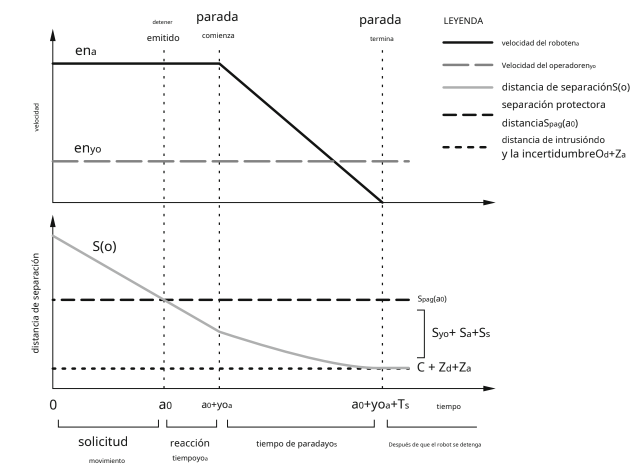
\includegraphics[width=0.7\textwidth]{Representacion_distancia_protectora.png}
  \caption{Contribuciones a la distancia de separación protectora entre operador y robot. Información adaptada de \cite{lenarcic2012}.}
  \label{fig:separacion}
\end{figure}

\begin{figure}[htbp]
  \centering
  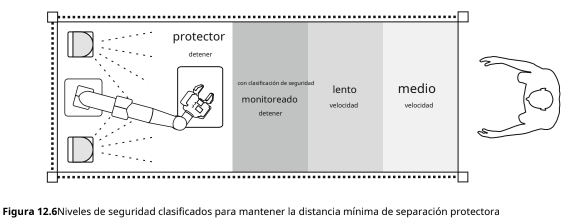
\includegraphics[width=0.6\textwidth]{niveles de seguridad.png}
  \caption{Niveles de seguridad para mantener la distancia mínima de separación protectora. Información adaptada de \cite{lenarcic2012}.}
  \label{fig:niveles-seg}
\end{figure}

\subsection{Limitación de potencias y fuerza}

El método de limitación de potencia y fuerza permite el contacto físico entre el sistema robótico y el operador, que puede producirse de forma intencionada o no. El método exige que los robots estén diseñados específicamente mediante baja inercia, geometría adecuada (bordes y esquinas redondeados, superficies lisas y flexibles), materiales (acolchado, amortiguación, componentes deformables) y funciones de control \cite{lenarcic2012}. Hay dos tipos posibles de contacto: cuasiestático (sujeción o aplastamiento) y transitorio (contacto breve, menor a 50\,ms).

\begin{figure}[htbp]
  \centering
  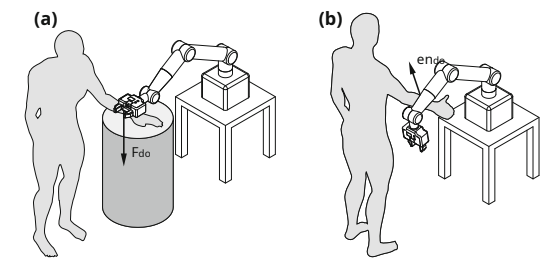
\includegraphics[width=0.6\textwidth]{interaccion_humano_robot Nota. a) Cuasi-estático y b) Contacto transitorio.png}
  \caption{a) Contacto cuasiestático y b) Contacto transitorio. Información adaptada de \cite{lenarcic2012}.}
  \label{fig:contacto}
\end{figure}

\section{Motor HerkuleX DRS 0602}

El servomotor HerkuleX DRS-0602 es un actuador modular inteligente que integra motor, reductor de engranajes, circuitos de control y capacidad de comunicación en un solo paquete, diseñado específicamente para aplicaciones que requieren alta precisión y durabilidad. Este servomotor cuenta con un codificador magnético basado en potenciómetro aplicado, que garantiza una alta resolución de 12\,960 pasos y excelente linealidad, aumentando las capacidades de control preciso y estable. Además, su diseño permite tanto una rotación continua como un ángulo de operación de hasta 900 grados, manteniendo una velocidad constante a través de su controlador de velocidad incorporado. Compacto y ligero, el DRS-0602 es ideal para robótica móvil y sistemas embebidos en los que la repetitividad, la durabilidad y la integración eficiente de componentes resultan esenciales para su óptimo funcionamiento.

\begin{figure}[htbp]
  \centering
  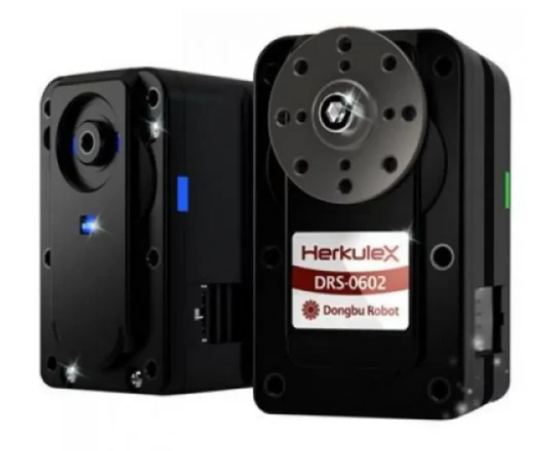
\includegraphics[width=0.5\textwidth]{motor_herk_1.png}
  \caption{HerkuleX DRS-0602 Smart Robot Servo. Información adaptada de RobotShop.}
  \label{fig:drs0602}
\end{figure}

\begin{figure}[htbp]
  \centering
  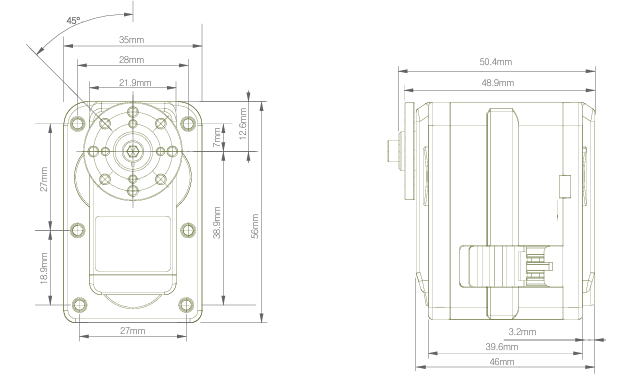
\includegraphics[width=0.5\textwidth]{Dimensiones de HerkuleX DRS-0602 .png}
  \caption{Dimensiones de HerkuleX DRS-0602 Smart Robot Servo. Información adaptada del manual.}
  \label{fig:drs0602-dim}
\end{figure}

\section{Gripper piCOBOT}

El gripper piCOBOT es un avanzado dispositivo de agarre diseñado específicamente para aplicaciones en robótica colaborativa. Desarrollado por la empresa Piab, se caracteriza por su diseño compacto, flexible y altamente adaptable, lo que lo convierte en una solución ideal para operar en colaboración con seres humanos en diversos entornos industriales. Su enfoque principal es ofrecer una herramienta segura y precisa, adecuada para cobots y otras aplicaciones robóticas que requieren estos atributos.

El piCOBOT cuenta con una unidad eyectora de vacío con controles integrados, indicadores visuales de estado de gran tamaño y una pantalla fácil de utilizar. Está disponible con una interfaz eléctrica genérica y ofrece varias opciones para las dimensiones de la placa de montaje mecánica, de acuerdo con la norma ISO 9409-1, lo que permite configurarlo para funcionar con cualquier robot colaborativo o robots industriales más pequeños. Certificado por Universal Robots, el piCOBOT se monta directamente en el brazo de los robots UR, cumpliendo con la norma ISO-9409-1-50-M6. Además, permite la opción de montar una ventosa directamente en la interfaz de rosca piCOBOT, o también es posible conectar una pinza ajustable de alta gama con dos ventosas para una mayor versatilidad. El dispositivo está equipado con un software complementario (URCaps) para el teach pendant (dispositivo de programación), lo que facilita su instalación, configuración y uso, permitiendo una rápida integración en cualquier entorno colaborativo.

\begin{figure}[htbp]
  \centering
  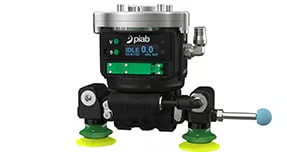
\includegraphics[width=0.5\textwidth]{efector_picobot.png}
  \caption{piCOBOT vacuum gripper unit. Información adaptada de Piab.}
  \label{fig:picobot}
\end{figure}

%% ============================================================================
%% CAPÍTULO 3 - DESARROLLO (Propuesta de desarrollo)
%% ============================================================================

\chapter{PROPUESTA DE DESARROLLO}

En este capítulo se detallan las actividades desarrolladas para cumplir con cada uno de los objetivos específicos planteados, así como las herramientas y técnicas empleadas durante el proceso.

\section{Investigación y puesta en marcha de los motores}

Los servomotores Herkulex DRS-0602, fabricados por Dongbu Robot, son actuadores inteligentes diseñados para aplicaciones en robótica que requieren control preciso de posición, velocidad y torque. Estos motores integran en un mismo módulo el motor DC, el controlador y un sistema de comunicación serial, lo que permite su gestión mediante comandos digitales.

De forma nativa, los servomotores Herkulex se comunican a través de un protocolo UART Multi Drop TTL, descrito por el fabricante como Full Duplex debido a la existencia de líneas diferenciadas de entrada (DIN) y salida (DOUT). Aunque, en configuraciones donde varios actuadores comparten el mismo bus de datos, la comunicación se comporta en la práctica como Half Duplex, ya que únicamente un dispositivo transmite en un instante determinado (Figura~\ref{fig:halffull}).

Para establecer la conexión con una computadora, se utiliza un dispositivo intermedio denominado Herkulex Manager Kit, el cual actúa como interfaz entre el bus de servomotores y el puerto USB de la PC. Esto permite controlar y configurar los motores mediante el software nativo Herkulex Manager, desarrollado por Dongbu Robot. A través de esta interfaz, el software detecta automáticamente los actuadores conectados, posibilitando la realización de tareas de diagnóstico, calibración, asignación de ID y prueba de movimiento.

En este proyecto, debido a la ausencia del Herkulex Hub, se implementó una solución alternativa para establecer la comunicación con los motores. Para ello, se utilizó una placa Arduino Uno modificada, de la cual se retiró el microcontrolador ATmega328P con el fin de aprovechar exclusivamente el módulo de conversión USB--Serial, basado en el chip ATmega16U2. De esta manera, la placa Arduino funcionó como un adaptador USB--TTL, permitiendo la conexión directa entre la PC y el bus de los servomotores, y posibilitando el uso del software Herkulex Manager sin requerir hardware propietario adicional. Esta adaptación permitió la inicialización, reconocimiento y control de los motores Herkulex desde la computadora, reproduciendo parcialmente las funcionalidades del hub original y sirviendo como base para el desarrollo posterior del sistema de control personalizado.

Durante la puesta en marcha se detectaron limitaciones en el software Herkulex Manager, específicamente al intentar modificar los identificadores (ID) de los motores. Si bien el programa permitía realizar la asignación, los valores no se almacenaban de forma persistente, y al reiniciar los servomotores estos retornaban al ID por defecto (256). Para superar esta dificultad, se desarrolló un código en Python que permitió enviar los comandos de configuración directamente a través del puerto serial. Este desarrollo incluyó la creación de una librería propia, dado que las bibliotecas disponibles en línea estaban orientadas a modelos anteriores de la serie Herkulex, tales como los DRS-0101 y DRS-0601, los cuales presentan diferencias significativas en su protocolo de comandos. La nueva librería se diseñó específicamente para el modelo DRS-0602, considerando sus particularidades y limitaciones, y permitió establecer comunicación estable, modificar IDs de forma permanente y ejecutar movimientos básicos mediante comandos personalizados.

En cuanto a la alimentación eléctrica, los servomotores Herkulex DRS-0602 operan dentro de un rango de tensión comprendido entre 9,5\,V y 15\,V, siendo 12\,V el valor óptimo de funcionamiento recomendado por el fabricante. Cada actuador incorpora su propio circuito de control y regulación interna, por lo que resulta fundamental garantizar una fuente de alimentación estable y libre de ruidos, capaz de suministrar la corriente necesaria para el conjunto de motores conectados. Dado que la corriente demandada por cada servomotor puede alcanzar valores del orden de 900\,mA en condiciones de carga máxima, se optó por alimentar los motores mediante una fuente externa dedicada, independiente de la utilizada para la lógica de control. No obstante, se mantuvo una referencia común de tierra (GND) entre la fuente de potencia, la interfaz de comunicación y la computadora, con el fin de asegurar niveles lógicos coherentes en las señales UART TTL.

\begin{figure}[htbp]
  \centering
  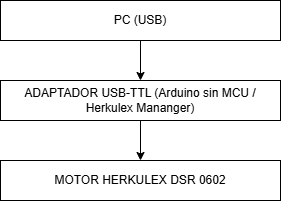
\includegraphics[width=0.7\textwidth]{Esquema_comunicacion.png}
  \caption{Esquema de comunicación. Elaboración propia.}
  \label{fig:comunicacion}
\end{figure}

\begin{figure}[htbp]
  \centering
  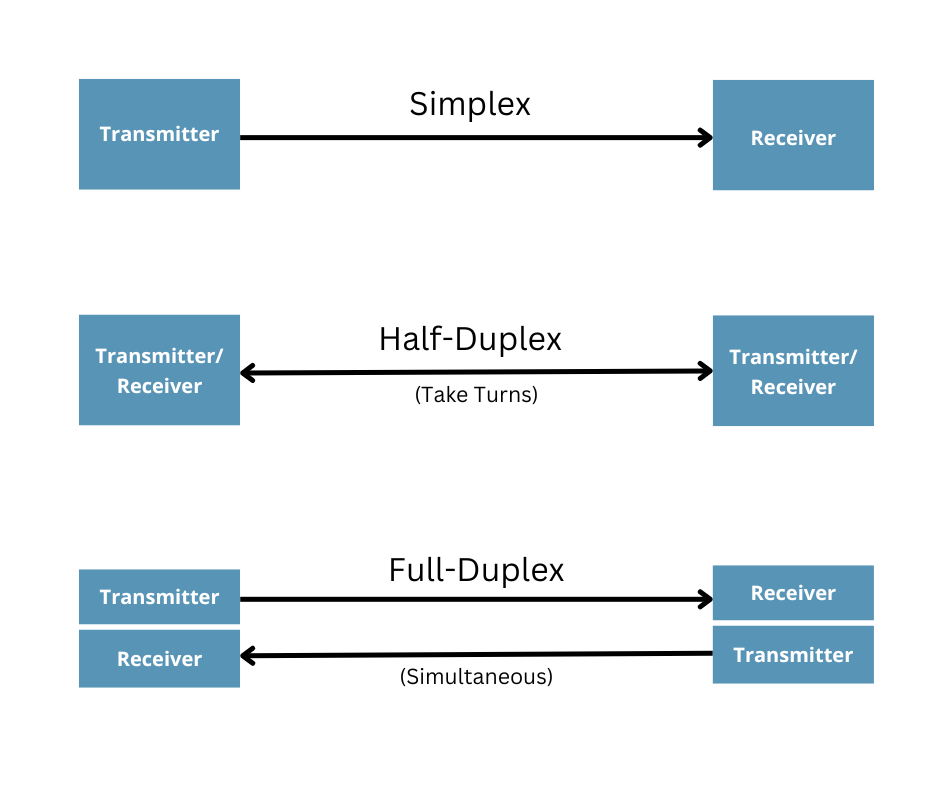
\includegraphics[width=0.6\textwidth]{images/Half-Duplex vs Full-Duplex.png}
  \caption{Half-Duplex vs Full-Duplex. Adaptado de Total Phase.}
  \label{fig:halffull}
\end{figure}

\begin{figure}[htbp]
  \centering
  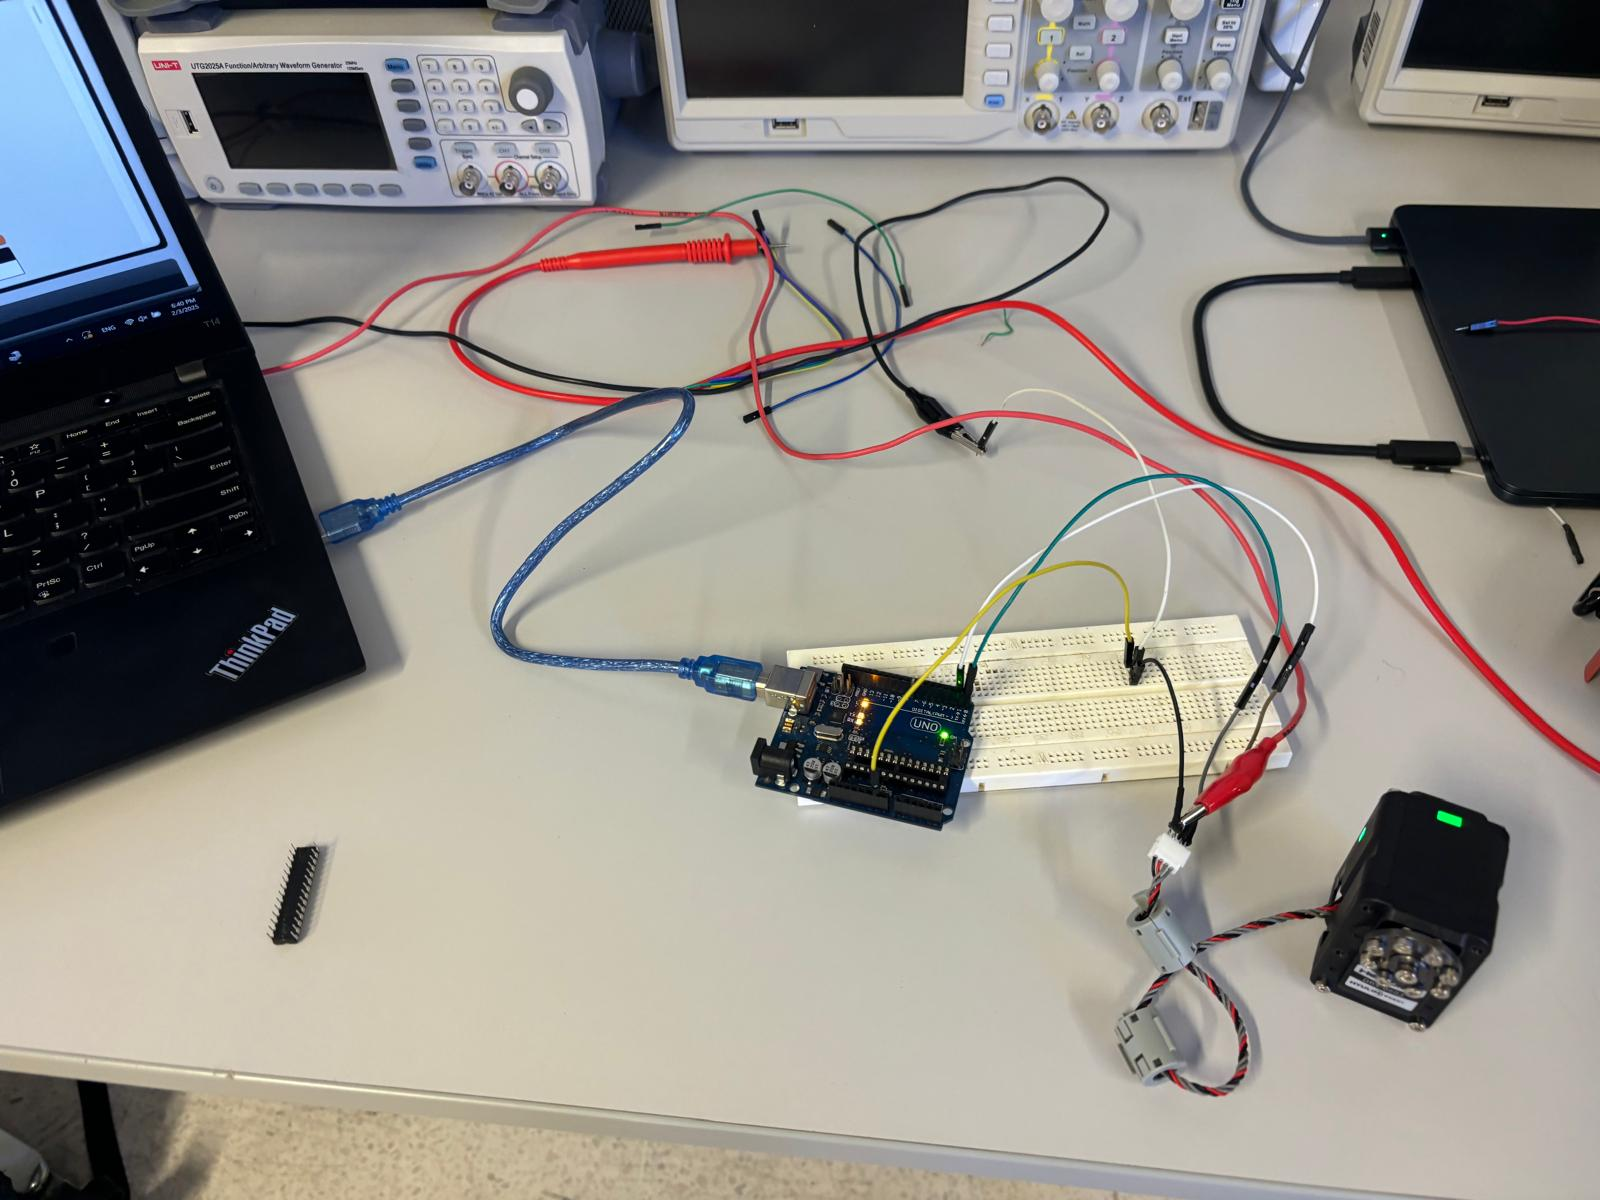
\includegraphics[width=0.6\textwidth]{evidencia de proceso.jpg}
  \caption{Diagrama de conexiones y evidencia de proceso. Elaboración propia.}
  \label{fig:conexiones}
\end{figure}

\section{Diseño y desarrollo}

\subsection{Introducción al diseño}

El diseño del cobot tuvo como propósito desarrollar una estructura compacta, modular y mecánicamente estable, capaz de alojar los servomotores Herkulex DRS-0602 respetando su geometría y rango de movimiento. Se buscó una configuración que maximizara el recorrido de cada articulación sin comprometer la rigidez del conjunto, manteniendo proporciones adecuadas para un brazo colaborativo de escritorio y garantizando condiciones seguras de operación.

Dado que el proyecto se enmarca en el desarrollo de un prototipo demostrativo, el enfoque de diseño se centró en lograr una solución simple, accesible y reproducible, capaz de evidenciar los principios básicos de movimiento, control y colaboración entre humano y robot. El diseño no solo buscó satisfacer los requerimientos técnicos del sistema (como el número de grados de libertad, la disposición de los actuadores o la precisión de los movimientos), sino también cumplir con las características esenciales de un robot colaborativo, tales como la seguridad, la suavidad de los bordes, el bajo peso y la limitación de velocidades y esfuerzos.

\subsection{Búsqueda de referencias y análisis de soluciones existentes}

Antes de iniciar el modelado del cobot, se realizó una búsqueda de diseños y desarrollos previos con el objetivo de comprender diferentes enfoques de construcción y soluciones mecánicas aplicadas en brazos robóticos. Se analizaron tanto prototipos académicos y de código abierto disponibles en repositorios en línea (Thingiverse, GrabCAD o CrealityCloud) como robots colaborativos comerciales, entre ellos el KUKA LBR iiwa, el Franka Emika Panda y el Universal Robots UR3.

El análisis de estos modelos permitió identificar distintos métodos de ensamblaje y transmisión de movimiento, así como estrategias de diseño estructural para optimizar la rigidez, el peso y la facilidad de mantenimiento. Si bien los cobots comerciales sirvieron como referencia conceptual en términos de proporciones, geometría y acabados, la implementación mecánica debió ser completamente original, debido a las diferencias en tamaño, componentes y en particular a la utilización de los servomotores Herkulex DRS-0602, para los cuales no existían referencias de integración disponibles.

\subsection{Requerimientos de diseño}

El proceso de diseño del cobot se consolidó a partir de los lineamientos definidos en las etapas previas. Se determinaron los requerimientos técnicos, de seguridad y constructivos que guiaron las decisiones de diseño, fabricación y montaje del sistema. Dado el carácter experimental y demostrativo del proyecto, se optó por fabricar la estructura mediante impresión 3D, priorizando la facilidad de iteración, el bajo costo y la rapidez de producción frente a la resistencia estructural. En esta etapa se seleccionó el material PLA, por su disponibilidad, facilidad de uso y buena estabilidad dimensional.

\begin{table}[htbp]
  \centering
  \caption{Tabla de requerimientos de diseño. Elaboración propia.}
  \label{tab:requerimientos}
  \small
  \begin{tabular}{p{2.2cm}p{3.5cm}p{6.5cm}}
    \toprule
    Categoría & Requerimiento & Descripción \\
    \midrule
    Técnico & Grados de libertad (4 DOF) & Al menos cuatro ejes articulados para movimientos básicos. \\
    & Integración Herkulex DRS-0602 & Montaje preciso, acoples personalizados. \\
    & Comunicación y cableado & Cableado TTL sin interferir con el movimiento. \\
    \midrule
    Seguridad & Movimiento colaborativo & Velocidades y torques limitados. \\
    & Geometría & Superficies redondeadas, sin bordes filosos. \\
    & Zona de trabajo & Alcance máximo adecuado. \\
    \midrule
    Constructivo & Pasaje interno de cables & Canalización para alimentación y señal. \\
    & Modularidad & Módulos reemplazables. \\
    \bottomrule
  \end{tabular}
\end{table}

\subsection{Diseño conceptual y modelado 3D}

El diseño conceptual del cobot se desarrolló a partir del análisis de diferentes modelos de brazos robóticos. El modelado tridimensional se realizó utilizando el software Autodesk Fusion 360, herramienta que permitió definir la geometría de cada componente y evaluar el movimiento relativo entre los ejes. Durante esta etapa se diseñaron las piezas principales que conforman el sistema: la base, los eslabones intermedios, las carcasas de motor y el extremo operativo. Se diseñó de forma modular, donde cada componente puede modificarse o reemplazarse de forma independiente. El resultado final fue un modelo tridimensional de cuatro grados de libertad (4 DOF), diseñado para operar sobre una superficie reducida y servir como plataforma demostrativa para la etapa de programación y control.

\subsection{Impresión 3D y ensamblaje del prototipo}

Construcción del prototipo mediante impresiones 3D, montaje, cableado y ensamblaje. Pruebas iniciales y ajustes realizados para validar el funcionamiento del cobot.

%% ============================================================================
%% CAPÍTULO 4 - RESULTADO Y ANÁLISIS
%% ============================================================================

\chapter{RESULTADO Y ANÁLISIS}

En este capítulo se presentan y analizan los resultados obtenidos según cada objetivo específico planteado, incluyendo el sistema de control, las pruebas de movimiento y la validación funcional del cobot.

\section{Introducción al sistema de control}

% Describa la arquitectura del sistema de control desarrollado (PC, Arduino, servomotores).
% Incluya diagramas si corresponde.

\section{Comunicación entre PC y servomotores}

% Presente los resultados de la comunicación entre la PC y los servomotores Herkulex DRS-0602.
% Incluya pruebas de estabilidad, asignación de IDs, etc.

\section{Desarrollo del software de control}

% Describa el software desarrollado (Python, Arduino, interfaz gráfica si aplica).
% Incluya capturas de pantalla o diagramas de flujo.

\section{Pruebas de movimiento y validación funcional}

% Presente los resultados de las pruebas de movimiento del cobot.
% Incluya secuencias de poses, calibración de motores, validación del gripper piCOBOT.
% Añada figuras o tablas con datos de las pruebas.


% Conclusiones y recomendaciones
%% ============================================================================
%% CONCLUSIONES
%% ============================================================================

\conclusions{%
Las conclusiones deben presentarse en forma de una lista numerada, con oraciones claras y breves que destaquen los principales resultados. Solo se incluirán aspectos analizados en el estudio y discutidos en los capítulos anteriores, permitiendo determinar si se alcanzaron los objetivos planteados.

\begin{enumerate}
  \item Se diseñó y construyó un cobot utilizando los motores Herkulex DRS-0602 y el gripper piCOBOT, cumpliendo con el objetivo general del proyecto.
  \item Se desarrolló una librería propia para el control de los servomotores DRS-0602, superando las limitaciones del software Herkulex Manager.
  \item La estructura modular en PLA permitió validar la integración mecánica y electrónica del prototipo de forma económica y reproducible.
  \item % Añada más conclusiones según los resultados obtenidos.
\end{enumerate}
}

%% ============================================================================
%% RECOMENDACIONES Y TRABAJOS FUTUROS
%% ============================================================================

\recommendations{%
Si se identifican oportunidades para ampliar o ajustar el trabajo realizado, o si se considera necesario modificar algún aspecto del proyecto, se incluirán aquí las recomendaciones y posibles trabajos futuros.

\begin{itemize}
  \item Utilizar materiales de mayor resistencia (ABS, aluminio) para aplicaciones industriales o de mayor durabilidad.
  \item Integrar el sistema de control en una placa embebida única (ESP32, Raspberry Pi) para mayor portabilidad.
  \item Desarrollar una interfaz gráfica de usuario para facilitar la programación de poses y secuencias por parte de los estudiantes.
  \item Poner el cobot a disposición de los alumnos para prácticas de robótica colaborativa.
  % Añada más recomendaciones según corresponda.
\end{itemize}
}


% Bibliografía (APA 7 - orden de aparición)
\renewcommand{\bibname}{\large\bf BIBLIOGRAFÍA}
\bibliographystyle{apalike}
\bibliography{referencias}

% Anexo
%% ============================================================================
%% ANEXO
%% ============================================================================

\appendix
\chapter{ANEXO}

Los anexos incluyen tablas y gráficas extraídas de libros, revistas o manuales técnicos que contribuyen a una mejor comprensión de la tesis. También abarcan aspectos clave de la implementación de programas informáticos, fotografías de equipos o productos, y planos de procesos o construcciones.

\section{Primera puesta en marcha}

\begin{figure}[htbp]
  \centering
  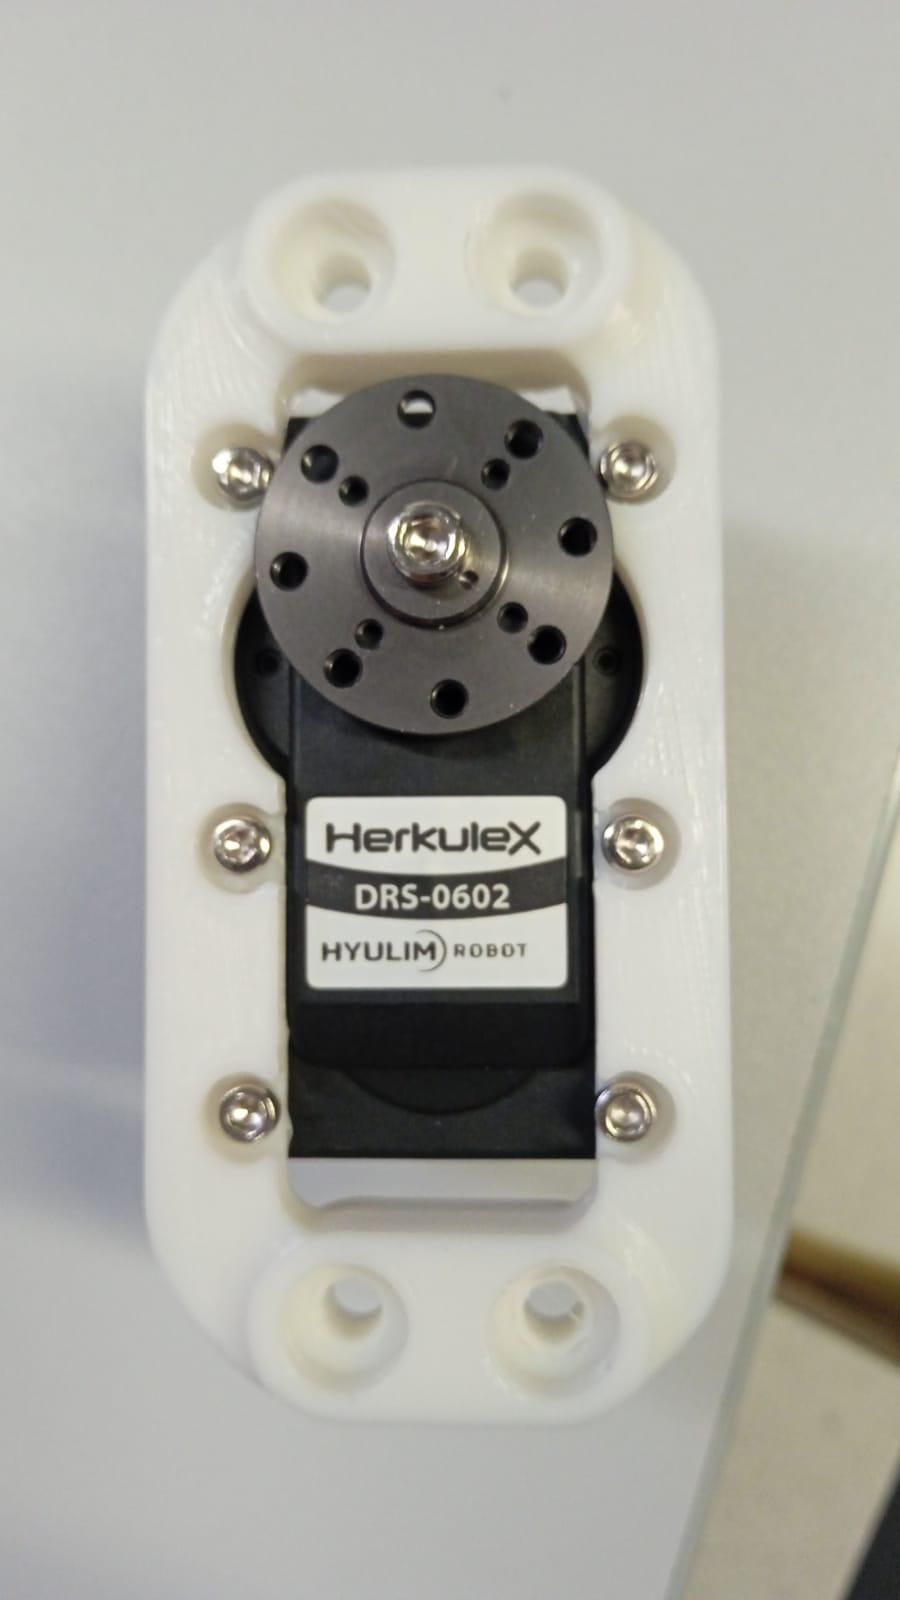
\includegraphics[width=0.7\textwidth]{ACOPLE ORIGINAL MOTOR.jpg}
  \caption{Acople original del motor.}
  \label{fig:anexo-acople}
\end{figure}

\section{Código y documentación}

% Referencia a la librería desarrollada: codigo/herkulex-drs0602-lib en el repositorio de la tesis.
% Incluya fragmentos de código relevantes si lo considera apropiado.


% Índices de tablas y figuras (al final, según template oficial)
\listoftables
\newpage
\listoffigures

\end{document}
%% ----------------------------------------------------------------
